\documentclass[usenames, dvipsnames, t]{beamer}

%\usepackage{geometry}
%\geometry{legalpaper, textwidth=426pt}
%\usepackage[T1]{fontenc}
%\usepackage{fourier}
\usepackage{graphicx}
%\graphicspath{{Figures/}}
%
\usepackage[english]{babel}															% English language/hyphenation
%\usepackage[protrusion=true,expansion=true]{microtype}
\usepackage{amsmath,amsfonts,amsthm} % Math packages
\usefonttheme[onlymath]{serif}
\usepackage{graphicx, adjustbox}
\graphicspath{{figures/}}
%\usepackage{url}
\newcommand{\red}[1]{\textcolor{red}{#1}}
\newcommand{\blue}[1]{\textcolor{blue}{#1}}
%
%% Self included packages
%%\usepackage[labelfont=sf,			hypcap=false,			format=hang,			width=\columnwidth]{caption}
%\usepackage{amsmath}
%\usepackage{wrapfig}
\usepackage[ruled, vlined]{algorithm2e}
\usepackage{pgfplots}
%\pgfplotsset{soldot/.style={color=blue,only marks,mark=*}} \pgfplotsset{holdot/.style={color=blue,fill=white,only marks,mark=*}}
\pgfplotsset{compat=1.12}
\usepackage{xcolor}
\usepackage{tikz}
\usetikzlibrary{graphs, graphs.standard, shapes.misc, positioning, fit, shadows, calc, snakes, shapes, patterns, arrows.meta, matrix, shapes.geometric}
% \usepackage[noend]{algpseudocode}
\usepackage{hyperref}
\hypersetup{
    colorlinks,
    citecolor=black,
    filecolor=black,
    linkcolor=black,
    urlcolor=black
}
%\usepackage{ifthen}
\usepackage{bm}
%\usepackage{enumerate}
%%%%%%%%%%%%%%%%%%%%%%%%%%%%%%%%%%%%%%%%%%%%%%%%%%%%%%%%%%%%%%%%%%%%%%%%%%%
\usetheme{CambridgeUS}
\usecolortheme{beaver}
\usepackage[english]{babel}

\setbeamertemplate{section in toc}{\inserttocsection}
\setbeamertemplate{subsection in toc}{\hspace{1.2em}~\inserttocsubsection\par}

\setbeamerfont{section in toc}{size=\small}
\setbeamerfont{subsection in toc}{size=\footnotesize}

\setbeamertemplate{itemize item}{\color{red}$\circ$}
\setbeamertemplate{itemize subitem}{\color{red}$\circ$}

\setbeamertemplate{enumerate item}[default]
\setbeamercolor*{enumerate item}{fg=red}
\setbeamercolor*{enumerate subitem}{fg=red}
\setbeamercolor*{enumerate subsubitem}{fg=red}

\setbeamertemplate{footline}
{
  \leavevmode%
  \hbox{%
  \begin{beamercolorbox}[wd=.2\paperwidth,ht=2.25ex,dp=1ex,center]{author in head/foot}%
  	\usebeamerfont{author in head/foot}\insertshortauthor
  \end{beamercolorbox}%

  \begin{beamercolorbox}[wd=.5\paperwidth,ht=2.25ex,dp=1ex,center]{title in head/foot}%
    	\usebeamerfont{title in head/foot}\insertshorttitle\hspace*{3em}
  \end{beamercolorbox}%

  \begin{beamercolorbox}[wd=.3\paperwidth,ht=2.25ex,dp=1ex,right]{date in head/foot}%
    	\usebeamerfont{date in head/foot}\insertshortdate{}\hspace*{2em}
	\insertframenumber{} / \inserttotalframenumber\hspace*{2ex}
  \end{beamercolorbox}}%
  \vskip0pt%
}

\title[Interpolation of MD with Bi-Directional NN]{Interpolation of Molecular Dynamics with Bi-Directional Neural Networks}
\subtitle{}
\author[Winkler \& Sauceda]{Ludwig Winkler \& Huziel Sauceda}
\date{\today}


%%%%%%%%%%%%%%%%%%%%%%%%%%%%%%%%%%%%%%%%%%%%%%%%%%%%%%%%%%%%%%%%%%%%%%%%%%%%
\begin{document}

\def\mathn#1{\mathnormal{#1}}
\def\thet{\bm{\theta}}
\def\V{\mathn{V}}
\def\Q{\mathn{Q}}
\def\R{\mathn{R}}
\def\r{\mathn{r}}
\def\G{\mathn{G}}
\def\n{\mathn{n}}
\def\A{\mathn{A}}
\def\T{\mathn{T}}
\def\W{\mathn{W}}
% \def\E{\mathbb{E}}

\def\w{\mathn{w}}
\def\p{\mathn{p}}
\def\q{\mathn{q}}
\def\a{\mathn{a}}
\def\r{\mathn{r}}
\def\s{\mathn{s}}
\def\t{\mathn{t}}
\def\dist{1}

\newcommand{\E}{\mathbb{E}}

\tikzset{ shorten <>/.style={ shorten >=#1, shorten <=#1 } }


\begin{frame}
	\titlepage
\end{frame}

% \begin{frame}
% \frametitle{Outline}
% \tableofcontents
% \end{frame}

\begin{frame}
	\frametitle{Molecular Dynamics (MD)}
	\begin{itemize}
		\item<+-> Molecules are governed by Newton's equations of motion 
		\item<+-> Position $r(t)$ and momentum $p(t)$ describe the system completely
		\item<+-> Dynamics $f$ given by differential equation (DiffEq)
		\begin{align*}
			\dot{x}(t) =
			\begin{bmatrix}
				\dot{r}(t) \\ 
				\dot{p}(t)
			\end{bmatrix}
			= f \left(
			\begin{bmatrix}
				r(t) \\ 
				p(t)
			\end{bmatrix}
			,t
			\right)
		\end{align*}
		\onslide<+->
		\item Solution is a trajectory in phase space
		\begin{align*}
			x(t) = 
			\begin{bmatrix}
				r(t) \\ 
				p(t)
			\end{bmatrix}
			= 
			\int_{t_0}^t f \left( \begin{bmatrix} r(t) \\ p(t) \end{bmatrix} ,t \right) dt
		\end{align*}
	\end{itemize}
\end{frame}

\begin{frame}
	\frametitle{Molecular Dynamics (MD)}
	\begin{itemize}
		\item<+-> High-dimensional N-body problems are expensive to solve
		\item<+-> MD requirements 
		\begin{itemize}
			\item $\Delta t = 10^{-15} s$ integration step size for accurate dynamics
			\item $T \in \{ 10^{-6} s, ...,  10^{-9} s \}$ solutions for expressive properties
		\end{itemize}
		\item<+-> Dynamics $f$ are expensive to compute for large N-body problems and long integration lengths
		\item[] 
		\item<+-> Yet, essentially we are dealing with a time series prediction problem ...
		\item[] 
	\end{itemize}
	\onslide<+->
		\begin{center}
		\textbf{Can we learn the phase space dynamics with a ML algorithm?}
		\end{center}
\end{frame}

\begin{frame}
	\frametitle{Learning Dynamical Systems}
	\begin{itemize}
		\item<+-> Given true dynamics $f$, learn dynamics $f_\theta$ with NN
		\item<+-> Optimize $f_\theta$ to predict the true solutions $x(t)$
		\item<+-> Integrate dynamics \red{$ \widehat{\dot{x}}(t) = f_\theta$} to obtain learned solution \red{$\hat{x}(t)$}
	\end{itemize}
	\onslide<+->
	\begin{figure}[!htbp]
		\begin{adjustbox}{max width = 0.3\textwidth, height = 0.4\textheight}
			\begin{tikzpicture}
				\tikzset{arrow/.style={-latex, shorten >= 5pt, shorten <= 5pt}}
				\tikzset{diff/.style={-latex, shorten >= 5pt, shorten <= 5pt}}
				\tikzset{node/.style={draw, circle, fill, scale=0.25}}
				
				% \clip (-0.5,3) rectangle (10,-3);

				\node (z0) [node]  at (0,-0.5) {}; 
				\node (zT) [node] at (5, 0.5) {};
		
				\draw[arrow, black] (z0.north) .. controls +(45:5cm) and +(225:5cm) .. (zT);
				\draw [decorate,decoration={brace,amplitude=10pt, mirror}, xshift=-4pt, yshift=0pt] (0,-1) -- (4.9,-1) node [black,midway,yshift=-0.6cm] {\large $x(t)$};
				
				\node (zT1) at (10, -0.5) {};
				\draw[draw=none] (zT.north) .. controls +(50:3cm) and +(225:3cm) .. (zT1)
				\foreach \t in {33,66,100}
				{ node[red] (a\t) [pos=\t/100,node,draw=red] {} };
				
				\draw[red, dotted, arrow] (zT) to node[below, red] {} (a33);
				\draw[red, dotted, arrow] (a33) to node[above right, red] {$\widehat{\dot{x}}(t)$}  (a66);
				\draw[red, dotted, arrow] (a66) to (a100);
		
				% \node (reala100)[node] at ($(a100)+(0,1.0)$) {};
				% \draw[black, dotted, arrow, shorten >= 2pt] (a66) to node[above, black] {\scriptsize $dx(t)$} (reala100);
				% \draw[{Bar[]}-{Bar[]}, red, dashed, shorten >= 3pt, shorten <= 3pt] (a100) to node[right]{$\mathcal{L}$} (reala100);
				\draw [red, decorate,decoration={brace,amplitude=10pt, mirror}, xshift=-4pt, yshift=0pt] (5.1,-1) -- (10,-1) node [red,midway,yshift=-0.6cm] {\large $\hat{x}(t)$};
		
				\node (zT2)[node] at (14, 1) {};
				\draw[arrow, black] (a100.east) .. controls +(20:2cm) and +(135:2cm) .. node[above left] {$x(t)$} (zT2);
				\draw [decorate,decoration={brace,amplitude=10pt, mirror}, xshift=-4pt, yshift=0pt] (10.1,-1) -- (13.9,-1) node [black,midway,yshift=-0.6cm] {\large $x(t)$};
				
				\node (zT3) at (18, 0.5) {};
				\draw[draw=none] (zT2.north) .. controls +(300:3cm) and +(225:3cm) .. node[above right, red]{} (zT3)
				\foreach \t in {33,66,100}
				{ node[red] (b\t) [pos=\t/100,node,draw=red] {} };
				
				% \draw[red, dotted, arrow] (zT2) to node[above right, red] {123} (b33);
				\draw[red, dotted, arrow] (zT2) to (b33);
				\draw[red, dotted, arrow] (b33) to (b66);
				\draw[red, dotted, arrow] (b66) to node[above left, red] {$\widehat{\dot{x}}(t)$} (b100);
		
				\draw [red, decorate,decoration={brace,amplitude=10pt, mirror}, xshift=-4pt, yshift=0pt] (14.1,-1) -- (18.1,-1) node [red,midway,yshift=-0.6cm] {\large $\hat{x}(t)$};
			
			\end{tikzpicture}
		\end{adjustbox}
		\end{figure}
\end{frame}

\begin{frame}
	\frametitle{Learning Dynamical Systems}
	\framesubtitle{Model Architectures}
	\begin{itemize}	
		\item<+-> ODENetwork
		\begin{align*}
			\dot{x}(t) =
			\begin{bmatrix}
				\dot{r}(t) \\ 
				\dot{p}(t)
			\end{bmatrix}
			= f \left(
			\begin{bmatrix}
				r(t) \\ 
				p(t)
			\end{bmatrix}
			,t
			\right)
		\end{align*}
		\item<+-> HamiltonianNetwork
		\begin{align*}
			\dot{x}(t) = 
	\begin{bmatrix}
		\dot{r}(t) \\ \dot{p}(t)) 
	\end{bmatrix}
		= 
		\begin{bmatrix}
		\ \ \frac{\partial \mathcal{H}(r(t), p(t), t)}{\partial p(t)} \\ - \frac{\partial \mathcal{H}(r(t), p(t), t)}{\partial r(t)}
		\end{bmatrix}
		\end{align*}
		\item<+-> LSTM performed best
		\item<+-> Due to fewest assumptions and flexible parameterization
	\end{itemize}
\end{frame}

\begin{frame}
	\frametitle{Learning Dynamical Systems with LSTM}
	\begin{itemize}
		\item LSTM uses memory cell $c(t)$ to selectively read and write information
		\item Outputs $[ \dot{r}(t), \dot{p}(t)]^T$ are integrated to obtain solution $\hat{x}(t)$
	\end{itemize}
	\begin{figure}
		% \centering
		\begin{adjustbox}{max width = 1.\textwidth, height = 0.6\textheight}
			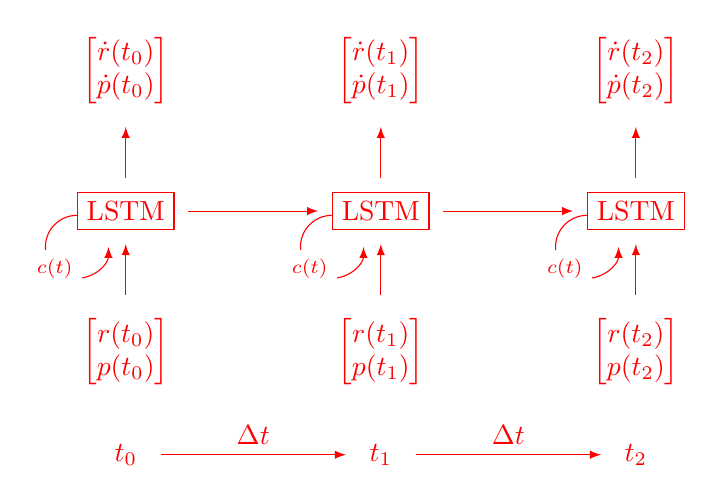
\begin{tikzpicture}[node distance=2cm]
				\tikzset{arrow/.style={-latex, shorten >= 5pt, shorten <= 5pt}}
				% \tikzset{diff/.style={-latex, shorten >= 5pt, shorten <= 5pt}}
				% \tikzset{node/.style={draw, circle, fill, red, scale=0.25}}
				\tikzset{LSTMCell/.style={draw, rectangle, red, scale=1.}}

				% \clip (-3,-4) rectangle (10,3);
				
				% Step 0
				\node (lstm0) [LSTMCell] at (0,0) {LSTM}; 
				\draw [-latex, red, draw] ([xshift=-0.0cm]lstm0.185) arc[radius=0.4cm, start angle=90, end angle=360] node[midway, red, fill=white](){\scriptsize $c(t)$};
				
				\node (input0) [red, below = 1cm of lstm0] {$\begin{bmatrix} r(t_0) \\ p(t_0) \end{bmatrix}$};
				\draw [arrow, red] (input0) -- (lstm0);
				\node (output0) [red, above = 1cm of lstm0] {$\begin{bmatrix} \dot{r}(t_0) \\ \dot{p}(t_0) \end{bmatrix}$};
				\draw [arrow, red] (lstm0) -- (output0);

				% Step 1
				\node (lstm1) [LSTMCell, right = of lstm0] {LSTM}; 
				\draw [-latex, red, draw] ([xshift=-0.0cm]lstm1.185) arc[radius=0.4cm, start angle=90, end angle=360] node[midway, red, fill=white](){\scriptsize $c(t)$};
				
				\node (input1) [red, below = 1cm of lstm1] {$\begin{bmatrix} r(t_1) \\ p(t_1) \end{bmatrix}$};
				\draw [arrow, red] (input1) -- (lstm1);
				\node (output1) [red, above = 1cm of lstm1] {$\begin{bmatrix} \dot{r}(t_1) \\ \dot{p}(t_1) \end{bmatrix}$};
				\draw [arrow, red] (lstm1) -- (output1);

				% Step 2
				\node (lstm2) [LSTMCell, right = of lstm1] {LSTM}; 
				\draw [-latex, red, draw] ([xshift=-0.0cm]lstm2.185) arc[radius=0.4cm, start angle=90, end angle=360] node[midway, red, fill=white](){\scriptsize $c(t)$};
			
				\node (input2) [red, below = 1cm of lstm2] {$\begin{bmatrix} r(t_2) \\ p(t_2) \end{bmatrix}$};
				\draw [arrow, red] (input2) -- (lstm2);
				\node (output2) [red, above = 1cm of lstm2] {$\begin{bmatrix} \dot{r}(t_2) \\ \dot{p}(t_2) \end{bmatrix}$};
				\draw [arrow, red] (lstm2) -- (output2);

				% Recurrent connections
				\draw [arrow, red] (lstm0) -- (lstm1);
				\draw [arrow, red] (lstm1) -- (lstm2);
				
				% Time Steps
				\node (t0)[red, below=0.5cm of input0]{$t_0$};
				\node (t1)[red, below=0.5cm of input1]{$t_1$};
				\node (t2)[red, below=0.5cm of input2]{$t_2$};
				\draw [arrow, red] (t0) -- node[above]{$\Delta t$} (t1);
				\draw [arrow, red] (t1) -- node[above]{$\Delta t$} (t2);
			
			\end{tikzpicture}
		% }
		\end{adjustbox}
	\end{figure}
\end{frame}

\begin{frame}
	\frametitle{Bi-Directional Interpolation of Differential Equation}
	\begin{itemize}
		\item Predict forward solution \red{$\overrightarrow{\hat{x}(t)}$} and backward solution \blue{$\overleftarrow{\hat{x}(t)}$} with the \textbf{same} dynamics $f_\theta$
		\item Use adiabatic connection to interpolate \red{$\overrightarrow{\hat{x}(t)}$} and \blue{$\overleftarrow{\hat{x}(t)}$} to $\hat{x}(t)$
		\begin{align}
			\hat{x}(t) = (1-\lambda(t)) \ \red{\overrightarrow{\hat{x}(t)}} + \lambda(t) \ \blue{\overleftarrow{\hat{x}(t)}}
		\end{align}
	\end{itemize}
	% \resizebox*{0.5\textwidth}{1.2\textheight}{
	\begin{figure}
		% \centering
		\begin{adjustbox}{max width = 1.\textwidth, height = 0.5\textheight}
			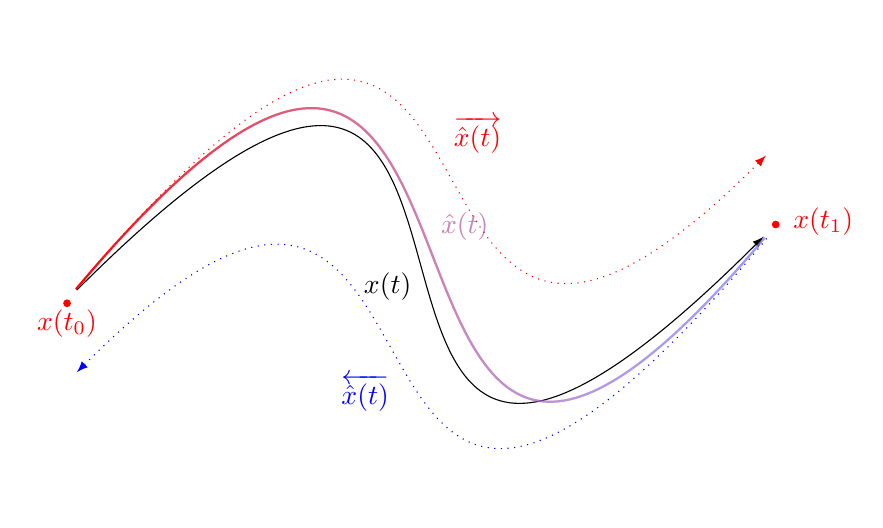
\begin{tikzpicture}
			\tikzset{arrow/.style={-latex, shorten >= 5pt, shorten <= 5pt}}
			\tikzset{diff/.style={-latex, shorten >= 5pt, shorten <= 5pt}}
			\tikzset{node/.style={draw, circle, fill, red, scale=0.25}}

			\clip (-0.5,3) rectangle (10,-3);
			
			\node (z0) [node, label={[below, red]{$x(t_0)$}}] at (0,-0.5) {}; 
			\node (zT) [node, label={[right=0.1cm, red]{$x(t_1)$}}] at (9, 0.5) {};
			\draw[arrow, black] (z0.north) .. controls +(45:10cm) and +(225:10cm) .. node[below left]{$x(t)$} (zT);
			\draw[shorten >= 5pt, shorten <= 5pt, , red, thick, path fading=east] (z0.north) .. controls +(50:10cm) and +(230:9.5cm) .. node[above right]{$\hat{x}(t)$} (zT);
			\draw[shorten >= 5pt, shorten <= 5pt, blue!50, thick, path fading=west, opacity=0.8] (z0.north) .. controls +(50:10cm) and +(230:9.5cm) .. node[above right]{$\hat{x}(t)$} (zT);
			
			\draw[arrow, dotted, red] (z0.north) .. controls +(50:10cm) and +(225:8cm) .. node[above right]{$\overrightarrow{\hat{x}(t)}$} ($(zT)+(0cm,1cm)$);
			
			% \draw[draw=none] (z0.north) .. controls +(50:10cm) and +(225:8cm) .. node[above right]{$\overrightarrow{\hat{x}(t)}$} ($(zT)+(0cm,1cm)$)
				% \foreach \t in {25, 50, 75, 90, 100}
					% { node[red] (forward\t) [pos=\t/100,node,draw=red] {} };
			
			% \draw[arrow, dotted, red] (z0) to (forward);
			% \foreach \s/\e in {25/50, 50/75, 75/90, 90/100}
			% 	{
			% 	\draw[arrow, dotted, red] (forward\s) to (forward\e);
			% 	}
			
			\draw[arrow, dotted, blue] (zT.south) .. controls +(230:10cm) and +(45:8cm) .. node[below left]{$\overleftarrow{\hat{x}(t)}$}($(z0)+(0cm,-1cm)$);
		
			\end{tikzpicture}
		% }
		\end{adjustbox}
	\end{figure}
\end{frame}

\begin{frame}
	\frametitle{Bi-Directional Interpolation of Differential Equation}
	\begin{itemize}
		 \item Unidirectional LSTM architecture for Benzene MD trajectory interpolating over 20 time steps
	\end{itemize}
	\begin{figure}
		 \centering
		 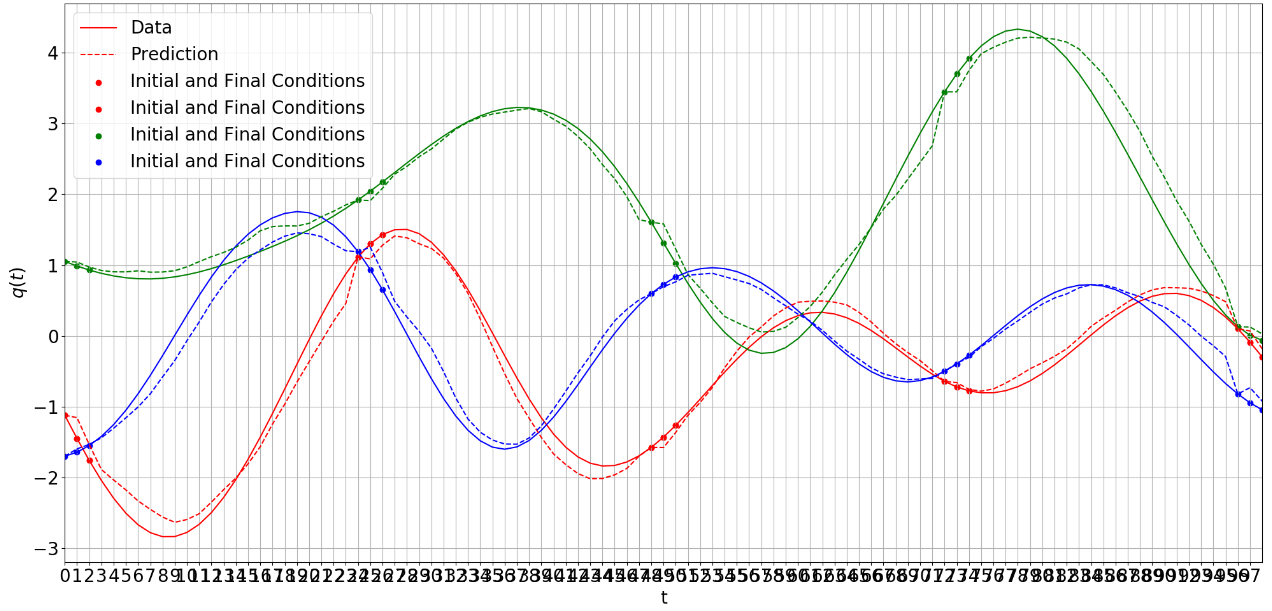
\includegraphics[width=0.8\textwidth]{ExampleTrajectory.png}
	\end{figure}
\end{frame}

\begin{frame}
	\frametitle{Bi-Directional Interpolation of Differential Equation}
	\begin{itemize}
		 \item Bidirectional LSTM architecture for Benzene MD trajectory interpolating over 20 time steps
		 \item Final condition and additional bidirectional training smooth trajectories significantely
	\end{itemize}
	\begin{figure}
		 \centering
		 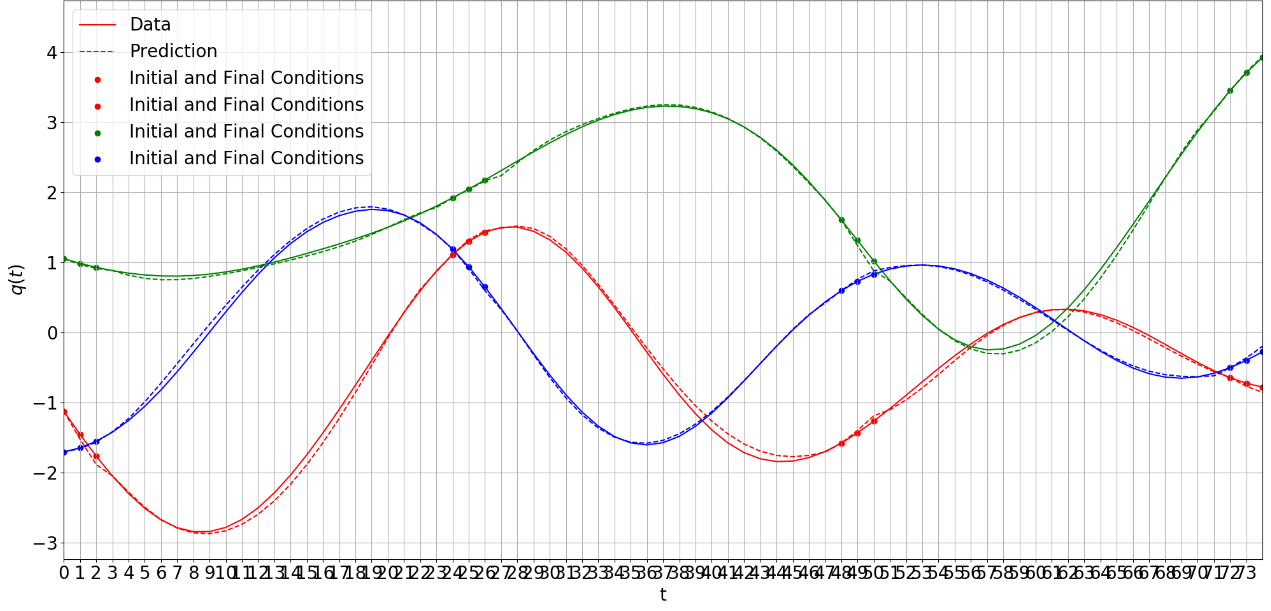
\includegraphics[width=0.8\textwidth]{ExampleTrajectoryBi.png}
	\end{figure}
\end{frame}

\begin{frame}
	\frametitle{Bi-Directional Interpolation of Differential Equation}
	\begin{itemize}
		 \item Single initial and final condition already good for sufficient performance by bidirectional LSTM
	\end{itemize}
	\begin{figure}
		 \centering
		 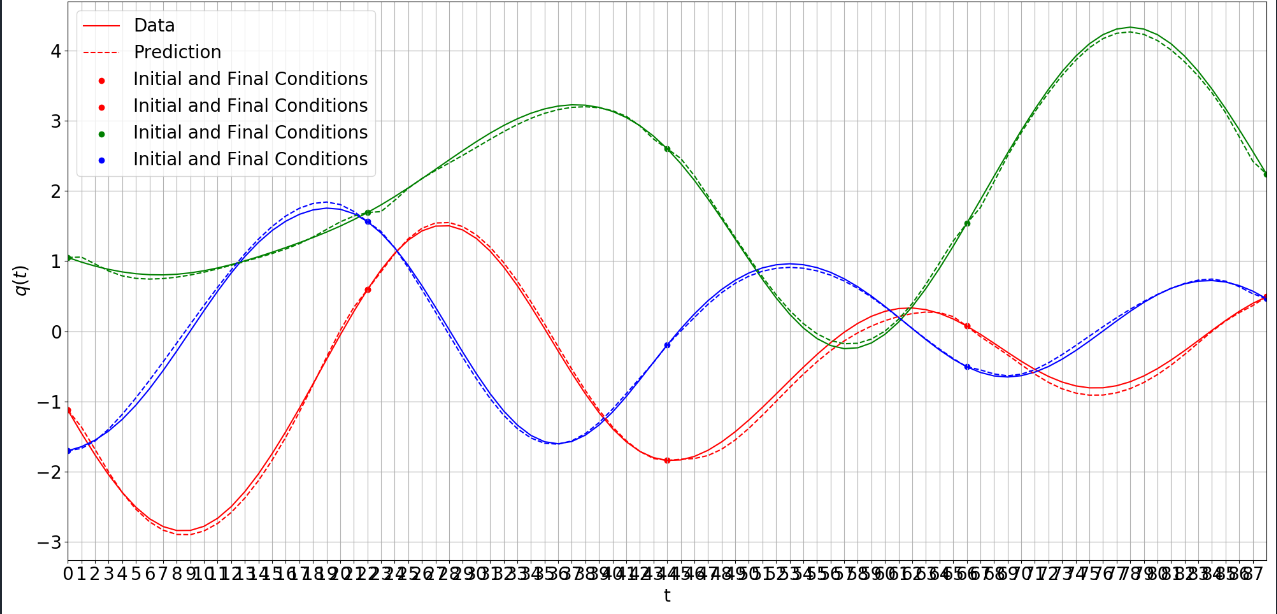
\includegraphics[width=0.8\textwidth]{ExampleTrajectoryBiIn1.png}
	\end{figure}
\end{frame}

\end{document}
